%!TEX root = ../diplom.tex
\section{Алгоритм ретрекинга}
\begin{figure}[h]
    \centering
    \def\svgwidth{0.8\linewidth}
    %\import{./fig/}{geometry.pdf_tex}
    \includesvg{geometry}
    \caption{Геометрия задачи вычисления отклика радиолокатора на плоскую
    поверхность с учетом отклонения антенны от надира.}
    \label{fig:geometry}
\end{figure}
Посчитаем теоретически отклик плоской морской поверхности $P_{FS}$ на сигнал с
радиолокатора.
Предполагаем известными диаграмму направленности $G(\theta)$, мощность
излученной энергии как функцию времени $P(t)$ и длину волны излучения
$\lambda$.

%Рассмотрим импульсный радиолокатор, который через равные или квазиравные
%промежутки времени подает  на антенну напряжение следующего вида
%\begin{equation}
    %\label{eq:U}
    %U(t) = 
    %\begin{cases}
        %\Re{\tilde U(t) e^{i \omega t}}, & \text{ при } t\geq 0 \\
        %0                         , & \text{ при } t<0.
    %\end{cases}
%\end{equation}

%Мощность такого сигнала будет равна
%\begin{equation}
    %\label{eq:}
    %P(t) = \frac{\tilde U(t)^2}{2}
%\end{equation}
%Поскольку радиолокатор излучает сферическую волну, её амплитуда будет
%уменьшаться по закону $\sim \frac{1}{r}$, 


Рассматривая малую плоскую площадку $m$, мы можем
составить уравнение, описывающее отраженную от неё мощность из следующих
четырех множителей:
\begin{equation}
    \label{eq:Pfsm}
    P_{FS_m} = 
    \frac
        {P\qty(t - \frac{2r_m}{c}) G_m}
        {4 \pi r_m^2} 
    \cdot \sigma^o_mA_m
    \cdot \frac{1}{4 \pi r_m^2} 
    \cdot \frac{G_m \lambda^2}{4 \pi}=
    \frac
        {P\qty(t - \frac{2r_m}{c})G_m^2 \lambda^2 \sigma^o_m}
        {(4 \pi)^3 r_{m}^4},
\end{equation} 
где 
$r_m$ -- расстояние от радара до рассеивающей площадки ,
$\sigma^o_m$ -- удельная эффективная площадь рассеяния площадки,
$G_m$ -- диаграмма направленности антенны в направлении на рассеивающую
площадку,
$A_m$ -- площадь площадки.

Первый множитель в уравнении  \eqref{eq:Pfsm}  соответствует плотности мощности
излучаемого сигнала. Второй множитель характеризует энергию падающего
излучения, которая переизлучается в направлении приемника, то есть эффективную
площадь рассеяния. Третий множитель
характеризует рассеяние в пространстве переизлученной мощности из-за
сферичности волны. Четвертый
коэффициент это апертура антенны.

%Форма функции $P_{FS}$ ... 

%Из работы \cite{moore-and-williams} 
Для того, чтобы найти полную мощность переизлученного сигнала от интересующей
нас поверхности,
разобьем всю поверхность на элементарные площадки $\dd A$ и проинтегрируем
по ним 

\begin{equation}
    P_{FS}(t) = \frac{\lambda^2\mean{\sigma^o}}{(4 \pi)^3 } \int\limits_{} 
    \frac
        {P\qty(t - \frac{2r}{c}) G^2(r,\theta,\phi) }
        {r^4} 
    \dd A
\end{equation}

 Из геометрии задачи (cм. рис. \ref{fig:geometry}) задачи можно найти связь между
 азимутальным углом $\theta$, полярными углами  $\phi$,  $\tilde \phi$ и
 отклонением антенны от положения надира
 \begin{equation}
     \label{eq:cos:theta}
     \cos \theta = 
     \frac{\cos \xi + \frac{\rho}{h} \sin \xi \cos(\tilde \phi - \phi)}{\sqrt{1
     + (\frac{\rho}{h})^2}}
 \end{equation}
 Поскольку боковые лепестки по мощности гораздо меньше главного лепестка, то
 пренебрежем ими и положим диаграмму направленности   равной следующей функции
 \begin{equation}
     \label{eq:Gapprox}
     G(\theta) = G_0 e^{-\frac{2}{\gamma} \sin^2 \theta}
 \end{equation}

 Подставим \eqref{eq:cos:theta} в \eqref{eq:Gapprox}, учтем, что  элемент
 поверхности можно записать как $\dd A = \rho \dd \rho \dd \psi$ и тогда
 интеграл преобразуется к виду  

 с учетом $r = \sqrt{h^{2} + \rho^{2}}$ 
 \begin{multline}
     P_{FS}(t) = \frac{G_0^2 \lambda^2}{(4 \pi)^3 h^4}
     \int\limits_{0}^{\infty} \int\limits_{0}^{2 \pi}   
     \frac{P\qty(t - \frac{2h}{c}\sqrt{1+ \epsilon^2})}{(1+\epsilon^2)^2} \sigma^o(\psi)
     \\
     \cdot \exp{-\frac{4}{\gamma} \qty[1 - \frac{\cos^2 \xi}{1+ \epsilon^2}] + b
     + a\cos(\tilde \phi - \phi) - b \sin^2(\tilde \phi - \phi)} \dd \phi \rho
     \dd \rho,
 \end{multline}
 где 
 $\epsilon = \frac{\rho}{h}$,
 $a = \frac{4\epsilon}{\gamma} \frac{\sin 2 \xi}{(1+ \epsilon^2)}$,
 $b= \frac{4\epsilon^2}{\gamma} \frac{\sin^2 \xi}{(1+\epsilon^2)}$,
 в рамках наших задач, нас не будет интересовать абсолютное значение мощности,
 а то его вид её зависимости от времени. 
 %Поэтому все константы можно
 %переобозначить как $A$.

 %поскольку интегрирование идет по полному периоду косинуса и синуса, то мы
 %можем игнорировать $\tilde \phi$. 

 %Разложим в ряд экспоненту по степеням $b\sin^2 \phi$, пользуясь малостью $b$
  %\begin{equation}
     %\label{eq:}
     %e^{- b \sin^2 \phi} = \sum\limits_{n=0}^{\infty} 
     %\frac{(-1)^2 b^n \sin^{2n}\phi}{n!}
 %\end{equation}
 Браун в своей работе \cite{brown} вычислил этот интеграл и показал, что он
 равен
 \begin{multline}
     \label{eq:}
     P_{FS} = \frac{G_0^2 \lambda^2 c}{4(4 \pi)^2 L_p h^3} \cdot
     \frac{\sigma^o(\psi)}{(\frac{ct}{2h})^3} 
     \cdot \exp{
         -\frac{4}{\gamma} 
         \qty[
         \cos^2 \xi - \frac{\cos 2\xi}{(\frac{ct}{2h})^2}
     ]}
     \\
     \cdot (1+\epsilon^2)^2\sum\limits_{n=0}^{\infty} \frac{(-1)^n
     \Gamma(n+\frac{1}{2})}{\sqrt \pi \Gamma(n+1)}\qty[\qty(\frac{ct}{2h})^2 -1
     \tan\xi]^n \\
     \cdot I_n \qty(\frac{4}{\gamma} \sqrt{\frac{c \tau}{n}} \sin 2 \xi),
     \text{ при } t\geq 2h /c
 \end{multline}
 и $P_{FS} = 0 \text{ при } t< 2h/c$


 Это выражение можно упростить, переходя к новому времени $\tau = t - 2h / c$,
 где  $2h / c$ -- время задержки между излучением и приемом сигнала. Учитывая,
 что в масштабах спутниковой альтиметрии  $\frac{c \tau}{h} \ll 1$, получим 

 \begin{multline}
     \label{eq:Pfs:final}
     P_{FS}(\tau) = \frac{G_0^2 \lambda^2 c \sigma^o(\psi_0)}{4(4 \pi)^2 L_p h^3}
     \exp{
         -\frac{4}{\gamma}\sin^2 \xi - \frac{4c}{\gamma h} \tau \cos 2 \xi
     }  \\
     \cdot \sum\limits_{n=0}^{\infty} \frac{(-1)^n \Gamma(n+\frac{1}{2})}{\sqrt
     \pi \Gamma(n+1)} \qty[\sqrt{\frac{c\tau}{h}}\tan \xi]^n
 I_n\qty(\frac{4}{\gamma} \sqrt{\frac{c \tau}{h}} \sin 2 \xi)
     \text{ при } \tau\geq 0
 \end{multline}
 и $P_{FS} = 0, \text{ при } \tau < 0$


 Рассмотрим теперь отдельно сумму из уравнения \eqref{eq:Pfs:final}. Если
 переобозначить $Y=\frac{4}{\gamma} \sqrt{\frac{c\tau}{h}} \sin 2\xi$, то сумма
 примет вид
 \begin{equation}
     \label{eq:sum}
     I_0(Y) \cdot \qty{ 1 + \sum\limits_{n=1}^{\infty} 
     \frac
        {(-1)^n \Gamma(n+\frac{1}{2})}
        {\sqrt \pi \Gamma(n+1)} 
        \cdot \frac{I_n(Y)}{I_0(Y)} \qty[\frac{\gamma Y}{8 \cos^2 \xi}]^n
 }
 \end{equation}
 Поскольку $Y\ll 1$ и $\xi \ll 1$, то множитель  $\qty[\frac{\gamma Y}{8 \cos^2
 \xi}]^n $ будет быстро сходиться к нулю. Следовательно сумму $n$ слагаемых мы
 можем приближенно заменить лишь одним слагаемым при $n=0$.
 \begin{multline}
     \label{eq:Pfs:approx}
     P_{FS}(\tau) = \frac{G_0^2 \lambda^2 c \sigma^o(\psi_0)}{4(4 \pi)^2 L_p h^3}
     \exp{
         -\frac{4}{\gamma}\sin^2 \xi - \frac{4c}{\gamma h} \tau \cos 2 \xi
     }  \\
     \cdot  I_0\qty(\frac{4}{\gamma} \sqrt{\frac{c \tau}{h}} \sin 2 \xi)
     \text{ при } \tau\geq 0
 \end{multline}

Можно прибегнуть к ещё одному упрощению и разложить в ряд функцию Бесселя в
уравнении \eqref{eq:Pfs:approx}:
\begin{equation}
    I_0(\zeta) = \sum\limits_{n=0}^{\infty} 
    \qty(\frac{\zeta^2}{4})^n \cdot 
    \qty(\frac{1}{n!})^2, \text{ где } \zeta=\frac{4}{\gamma}\sqrt{\frac{c \tau}{h}
    }\sin 2 \xi
\end{equation}
согласно статье \cite{amarouche} можно оставить только два первых члена
разложения, которые, в свою очередь, совпадают с разложением экспоненты
\begin{equation}
    I_0(\zeta) \approx 1 + \frac{\zeta^2}{4} = e^{\frac{\zeta^2}{4}}
\end{equation}
  
Тогда функция $P_{FS}$ примет вид
\begin{equation}
    \label{eq:Pfs}
    P_{FS}(\tau) = A \exp{-\frac{4}{\gamma} \sin^2 \xi} \exp{
        -\frac{4c}{\gamma h}
            \qty(\cos 2\xi - \sin^2 2\xi )\tau}
\end{equation}

 %Пропущу кусок
 %про 
 %Интегрируя почленно, получааем
 %\begin{multline}
     %\label{eq:}
     %P_{FS}(t) = 
     %\frac
        %{2 \sqrt \pi G_0 \lambda^2 \sigma^o(\psi_0)}
        %{(4 \pi)^3 L_p h^4}
     %\cdot\sum\limits_{n=0}^{\infty} 
     %\frac
     %{(-1)^n \Gamma(n+\frac{1}{2})}
     %{\Gamma(n+1)}\\
     %\cdot \int\limits_{0}^{\infty} \qty(\frac{2b}{a})^2 I_n(a) 
     %\cdot \exp{-\frac{4}{\gamma}\qty(1 - \frac{\cos^2 \xi}{1+
     %\epsilon^2})+b} 
     %\cdot \frac
     %{\delta\qty(t - \frac{2h}{c} \sqrt{1+ \epsilon^2})}
     %{(1+\epsilon^2)^2}
     %\rho \dd \rho,
 %\end{multline}
 %где $I_n(a)$ -- функция Бесселя, $\Gamma(n)$ -- гамма-функция Эйлера.



%Из геометрических соображений, можем определить что
%\begin{equation}
    %\label{eq:tanxi}
    %\tan \xi = \sqrt{\frac{c \tau}{h}}
%\end{equation}

Зная отклик плоской морской поверхности на сигнал с радиовысотомера мы
можем перейти к вычислению отклика на взволнованную морскую поверхность.
С точки зрения физики, различия будут в том, что теперь не вся
поверхность может отражать сигнал в нужном направлении, а только
зеркально ориентированные площадки на поверхности. С радиотехнической
точки зрения, взволнованная морская поверхность является линейным
фильтром с импульсной переходной характеристикой $q(t)$.  Тогда отклик
взволнованной поверхности можно вычислить выполняя свертку
\begin{equation}
    \label{eq:PRSconv}
    P_{RS}(t) = q(t) * P_{FS}(t) 
\end{equation}

Результирующая форму импульса будет сверткой функции отклика на плоскую
поверхность $P_{FS}$ и функции распределения зеркальных площадок $q$
 \begin{equation}
    \label{eq:}
    P(\tau) = \int\limits_{-\infty}^{\infty} q\qty(\tau
    -  \tilde\tau) P_{FS}(\tilde \tau) \dd{\tilde \tau} 
\end{equation}

Стоит заметить, что из-за малого значения параметра $\xi$ и  масштаба задачи 
$(c \tau)/h\ll 1$ функция $P_{FS}$ изменяется гораздо медленне функции плотности зеркальных точек $q$, а значит можно записать приближенное равенство \begin{equation}
    \label{eq:Psim}
    P \approx 
    \begin{cases}
        P_{FS}(0) \int\limits_{0}^{\infty} q\qty(\tau -
        \tilde \tau) \dd{\tilde \tau}, &\text{ при } \tau <0\\
        P_{FS}(\tau) \int\limits_{0}^{\infty} q\qty(\tau -
        \tilde \tau) \dd{\tilde \tau}, &\text{ при } \tau <0\\
    \end{cases}
\end{equation}

Поскольку корреляция между соседними площадками мала, а количество площадок
велико, то согласно
центральной предельной теореме мы можем положить распределение $q$ гауссовым
\begin{equation}
    \label{eq:q}
     q\qty(\tau) = 
        \frac
        {1}
        {\sqrt{2 \pi \qty(\frac{2 \sigma_s^2}{c})}}
    \exp{-\frac{\tau^2}{2 \pi \qty(\frac{2 \sigma_s^2}{c})^2}}
\end{equation}

%Посчитав свертку, получаем, что
%\begin{equation}
    %\label{eq:}
    %P(\tau) \approx P_{FS}(\tau) \qty[ 1 + \erf\qty(\frac{c\tau}{2 \sqrt 2 \sigma_s})]
%\end{equation}



%Согласно статье \cite{cite:moore-and-williams} можно связать дисперсию $\sigma_p$ в \eqref{eq:PTR} c
%временным разрешением альтиметра $r_t$:  
%\begin{equation}
    %\label{eq:sigmap}
    %\sigma_p = \frac{1}{2 \sqrt{2 \ln 2}} r_t
%\end{equation}

%Согласно работе Брауна  \cite{brown}, мы можем выразить $FSSR$ 

Напоследок, следует учесть, что наш приемник (радиолокатор) тоже является
линейной системой с некоторой импульсной характеристикой $P_{T}(t)$. Поэтому необходимо к
уравнению \eqref{eq:PRSconv} добавить ещё одну свертку. 
В работе \eqref{eq:moore-and-williams}  показано, что отклик радиолокатора
имеет гауссовую форму
\begin{equation}
    \label{eq:Pt}
    P_T(\tau) \sim \exp{-\frac{\tau^2}{2 \sigma_p^2}},
\end{equation}
где $\sigma_p = \frac{1}{\sqrt  2\ln 2} T \approx 0.425 T$, $T$ -- временное
разрешение антенны, по порядку величины обычно равное $T\sim 10$ нс.

Тогда, результирующий импульс будет равен
\begin{equation}
    \label{eq:Pconv}
    P(t) = P_{FS}(t) * q(t) * P_T(t)
\end{equation}
В свертке \eqref{eq:Pconv}, c учетом \eqref{eq:Pfs},\eqref{eq:Pt} и
\eqref{eq:q}, каждый множитель представляет собой экспоненту. Свертку от трех
экспонент не трудно посчитать аналитически. 

Получаем окончательную формулу для сигнала на приемнике радилокатора
\begin{equation}
    \label{eq:brown}
    P(t) = A e^{-v} (1 + \erf(u)), \text{ где}
\end{equation}
\begin{gather}
    A = A_0 \exp{\frac{- 4}{\gamma} \sin^2 \xi},\\
    u = \frac{t - \alpha \sigma_c^2}{\sqrt 2 \sigma_c},\\
    v = \alpha(t - \frac{\alpha}{2} \sigma_c^2),\\
\end{gather}
в которых

\begin{equation}
    \alpha = \delta - \frac{\beta^2}{4} = \frac{4}{\gamma}\cdot \frac{c}{h} \qty(\cos 2\xi - \frac{\sin^2 2\xi}{\gamma}),
\end{equation}
\begin{equation}
    \gamma = \frac{\ln 2}{2} \sin^2 \theta_{-3 dB},
\end{equation}
\begin{equation}
    \sigma_c^2 =  \sigma_p^2 + \frac{\sigma_s^2}{c^2},
\end{equation}
$\xi \ll 1$ -- малое отклонение антенны от надира,  $\theta_{-3 dB}$ -- ширина
диаграммы направленности антенны на уровне $-3dB$, $h$ -- высота радиолокатора
над поверхностью земли, $c$ -- скорость света в вакууме, $\sigma_s^2$ -- 
дисперсия высот взволнованной морской поверхности.



График функции \eqref{eq:brown} изображен на рис. \ref{fig:impuls}.

\subsection{Восстановление параметров морской поверхности.}%
\label{sub:vosstanovlenie_parametrov_morskoi_poverkhnosti_}

Зная зависимость принятого сигнала от параметров взволнованной морской
поверхности, мы можем восстанавливать их по форме импульса. Это можно сделать,
аппроксимируя практический импульс теоретической формулой и извлекая из
получившегося графика необхожимые коэффициенты.

Браун в своей работе вывел формулу, описывающего форму импульса в предположении
гауссовой плотности вероятности зеркальных площадок на морской поверхности.

Однако решать подобную задачу для формулы \eqref{eq:brown} довольно сложно
из-за сложной зависимости восстанавливаемых параметров и в  их большом
количестве.  Это может приводить к большим вычислительным ошибкам даже при большом соотношении сигнал-шум.

\begin{figure}[h]
    \centering
    \def\svgwidth{0.8\linewidth}
    \includesvg{impulse}
    \caption{Качественная форма импульса с обозначением основных параметров.}
    \label{fig:impuls}
\end{figure}

Поэтому для решения задачи ретрекинга предлагается, использовать менее физичную, но более наглядную запись формулы
\eqref{eq:brown}
\begin{equation}
    \label{eq:ice}
    P(t) = A \exp{ S_T (t - \frac{\tau}{2})} \qty(1 + \erf{\frac{t-
    \tau}{\sigma_L}}), \text{ где}
\end{equation}

$S_T$ -- коэффициент наклона заднего фронта импульса, 
 $\tau$ -- эпоха
 $\sigma_L$ -- ширина переднего фронта импульса, 

\paragraph{Поиск наклона заднего фронта.}%
\label{par:nakhozhdenie_s_t_}

Формула \eqref{eq:ice}, хороша тем, что можно найти некоторые коэффициенты, не
прибегая к сложным методам оптимизации. После прохождения пика импульса, функция ошибок
становится  медленно меняющейся функцией и можно записать равенство
\begin{equation}
    \label{eq:t>tmax}
    P(t) = 2A \exp{S_T \qty(t - \frac{\tau}{2})}, \text{ при } t > t_{max},
\end{equation}
где $t_{max}$ -- ордината пика импульса.

Логарифмируя \eqref{eq:t>tmax}
\begin{equation}
    \ln P(t) = \ln 2A + S_T( t - \frac{\tau}{2}) = S_T t + \const 
\end{equation}
мы получаем линейную функцию времени. Значит, построив логарифм формы импульса при
$t>t_{max}$ и найдя коэффициент наклона получившейся прямой мы можем найти
наклон заднего фронта $S_T$. Подобная процедура проведена на рис.\ref{fig:S_T}
 %\begin{figure}[h]
    %\centering
    %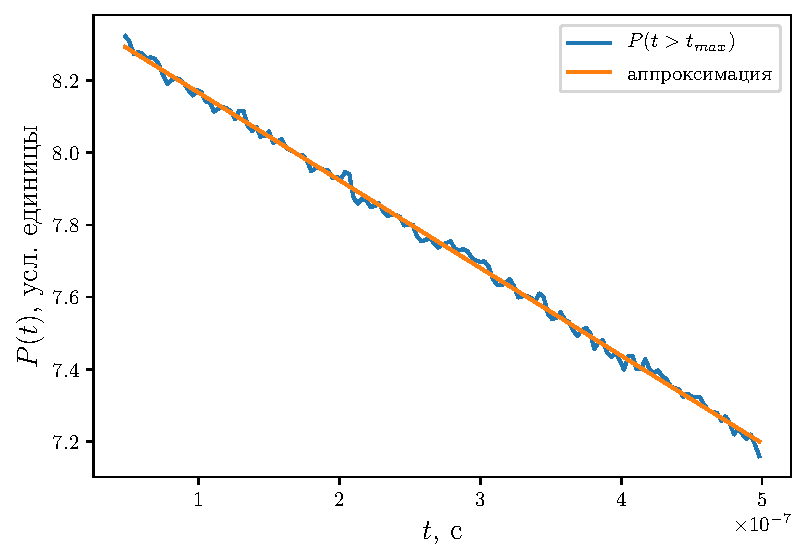
\includegraphics[width=\linewidth]{../project/radiolocator/imp08_7_1.pdf}
    %\caption{Нахождение наклона заднего фронта}
    %\label{fig:S_T}
%\end{figure}

\paragraph{Поиск ширины переднего фронта.}%
Как видно из рис.\ref{fig:erf}, при $t<t_{max}$ функция ошибок
$\erf\qty(\frac{t - \tau}{\sigma_L})$ ведет себя
быстрее экспоненты, а значит можно написать приближенное равенство
\begin{equation}
    \label{eq:erf}
    P(t) \approx A \qty(1 + \erf{\frac{t - \tau}{\sigma_L}})
\end{equation}

%\begin{figure}[h]
    %\centering
    %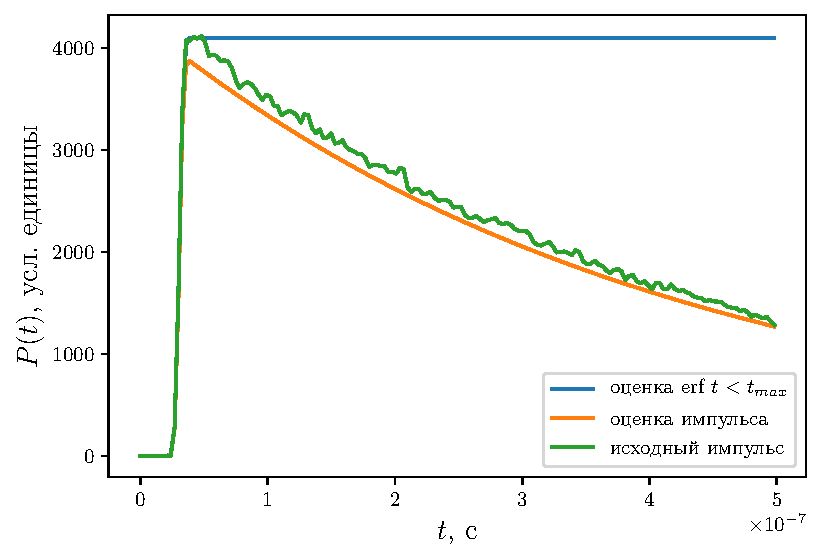
\includegraphics[width=\linewidth]{../project/radiolocator/imp08_7_2.pdf}
    %\label{fig:erf}
%\end{figure}

Аппроксимируя импульс при $t<t_{max}$ формулой \eqref{eq:erf} мы получим оценку
коэффициентов $A,~\tau,~\sigma_L$. 
%При этом, интересовать нас на этом этапе
%будут в основном  эпоха $\tau$ и ширина переднего фронта  $\sigma_L$.


 Имея оценки параметров аппроксимации по различным
участкам функции $P(t)$ мы можем использовать формулу  \eqref{eq:ice} для всего
импульса 
\begin{equation}
    \label{eq:ice}
    P(t) = A \exp{ S_T (t - \frac{\tau}{2})} \qty(1 + \erf{\frac{t-
    \tau}{\sigma_L}}).
\end{equation}
с начальными условиями для параметров $A, S_T, \tau, \sigma_L$, полученных на
предыдущих этапах. 


На рисунках ниже продемострированы результаты работы этого алгоритма на
различных формах импульса (меняются углы отклонения антенны).


\begin{figure}[ht]
    \begin{subfigure}{0.5\linewidth}
        \centering
        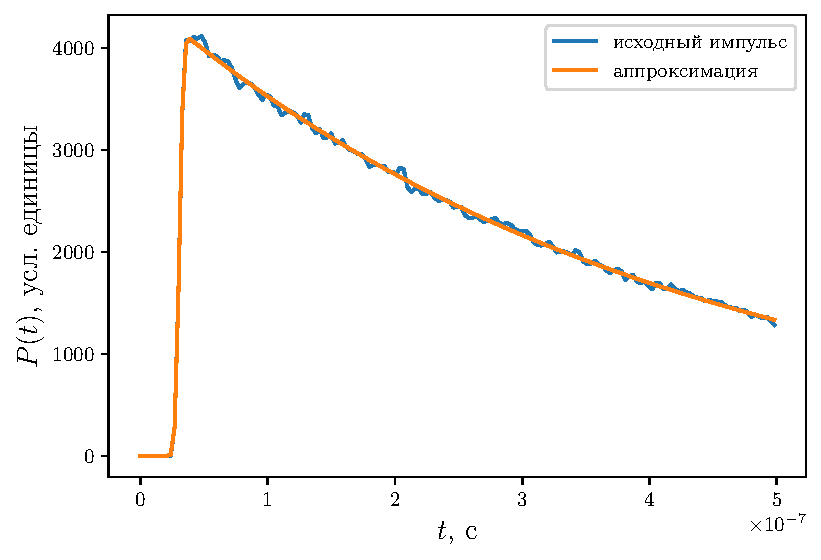
\includegraphics[width=\linewidth]{fig/retracking/imp08_7_3}
        \caption{Обработка файла imp08\_7.dat}
        \label{fig:}
    \end{subfigure}
    \begin{subfigure}{0.5\linewidth}
        \centering
        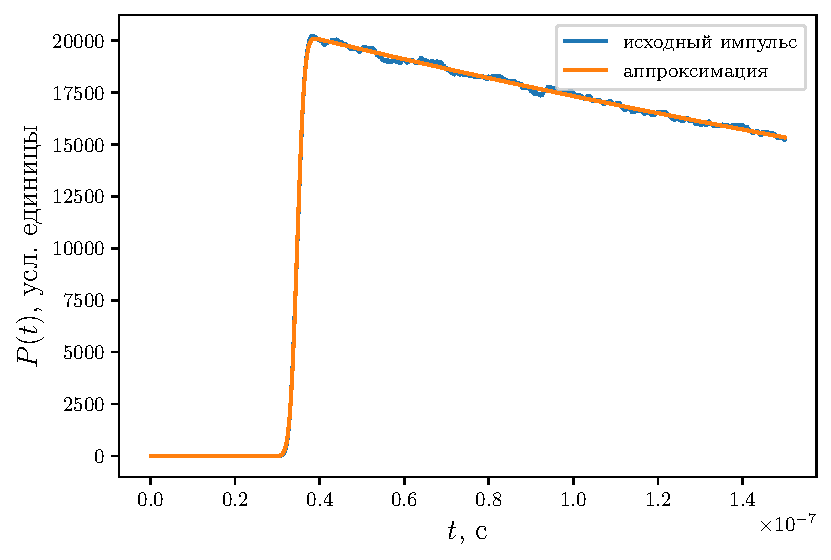
\includegraphics[width=\linewidth]{fig/retracking/imp_5_3}
        \caption{Обработка файла imp\_5.dat}
        \label{fig:}
    \end{subfigure}
    \begin{subfigure}{0.5\linewidth}
        \centering
        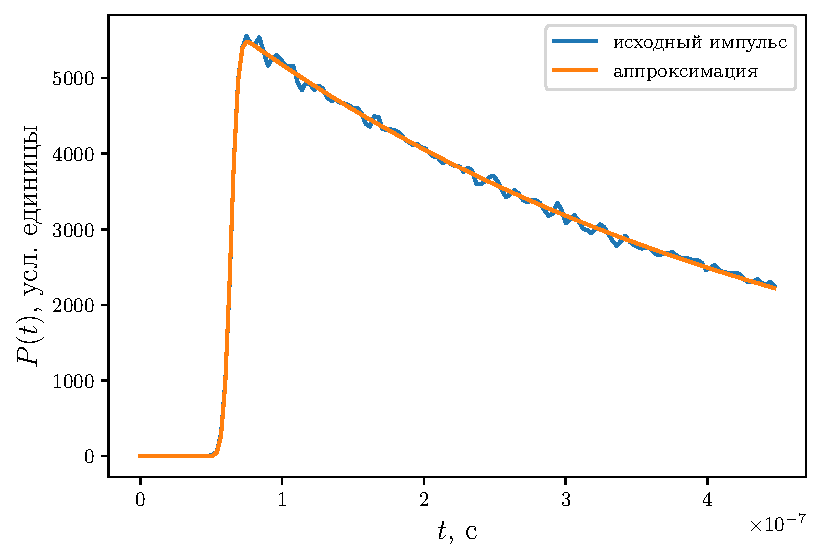
\includegraphics[width=\linewidth]{fig/retracking/imp04_10_3}
        \caption{Обработка файла imp04\_10.dat}
        \label{fig:}
    \end{subfigure}
    \begin{subfigure}{0.5\linewidth}
        \centering
        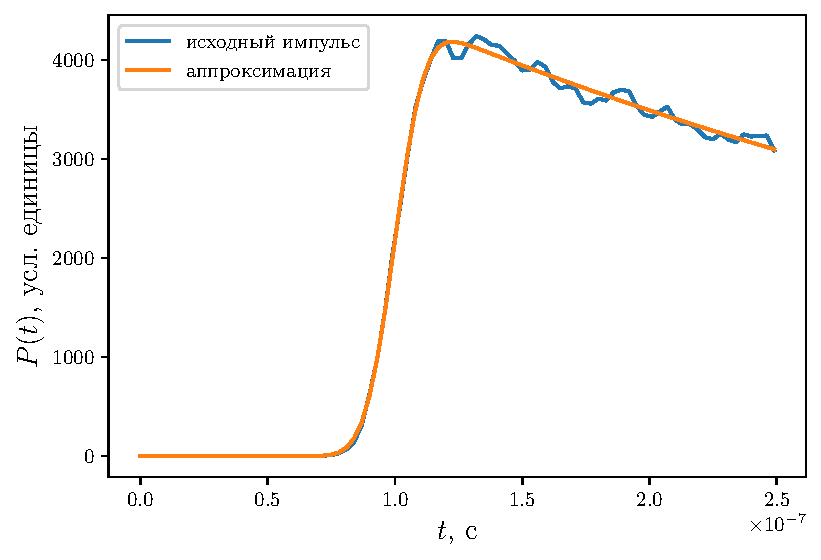
\includegraphics[width=\linewidth]{fig/retracking/imp_15a_3}
        \caption{Обработка файла imp15a.dat}
        \label{fig:}
    \end{subfigure}
\end{figure}






\paragraph{Восстановление параметров поверхности}%
Не сложно найти связь коэффициентов в формуле \eqref{eq:brown} и \eqref{eq:ice}:

\begin{equation}
    \label{eq:params}
    \begin{gathered}
        S_T = - \alpha,\\
        \sigma_L = \sqrt 2 \sigma_c,\\
        \sigma_c^2 = \sigma_p^2 + \frac{\sigma_s^2}{c^2}.
    \end{gathered}
\end{equation}

Из соотношений \eqref{eq:params} восстанавливается значение дисперсии высот
(высоты значительного  волнения). 
Из амплиитуды импульса мы можем узнать сечение обратного рассеяния, которое с
помощью различных моделей позволяет оценить скорость приводного ветра.



%Найдя коэффициенты для формулы \eqref{eq:ice} перейдем к формуле
%\eqref{eq:brown}
%и будем решать систему коэффициентов относительно неизвестных параметров
%радиовысотомера и состояния морской поверхности.

%\begin{gather}
    %A(A_0,\xi) = A_0 \exp{-\frac{4}{\gamma} \sin^2 \xi} \\
    %\alpha(\xi,h) = \frac{4c}{\gamma h} \cdot (\cos 2\xi - 
            %\frac{\sin^2 2\xi}{\gamma}) \\
    %\sigma_c^2 = \sigma_p^2 + \frac{\sigma_s^2}{c^2}
%\end{gather}


